\documentclass[twoside]{book}

% Packages required by doxygen
\usepackage{fixltx2e}
\usepackage{calc}
\usepackage{doxygen}
\usepackage{graphicx}
\usepackage[utf8]{inputenc}
\usepackage{makeidx}
\usepackage{multicol}
\usepackage{multirow}
\PassOptionsToPackage{warn}{textcomp}
\usepackage{textcomp}
\usepackage[nointegrals]{wasysym}
\usepackage[table]{xcolor}
\usepackage{ifpdf,ifxetex}

% Font selection
\usepackage[T1]{fontenc}
\usepackage[scaled=.90]{helvet}
\usepackage{courier}
\usepackage{amssymb}
\usepackage{sectsty}
\renewcommand{\familydefault}{\sfdefault}
\allsectionsfont{%
  \fontseries{bc}\selectfont%
  \color{darkgray}%
}
\renewcommand{\DoxyLabelFont}{%
  \fontseries{bc}\selectfont%
  \color{darkgray}%
}
\newcommand{\+}{\discretionary{\mbox{\scriptsize$\hookleftarrow$}}{}{}}

% Page & text layout
\usepackage{geometry}
\geometry{%
  a4paper,%
  top=2.5cm,%
  bottom=2.5cm,%
  left=2.5cm,%
  right=2.5cm%
}
\tolerance=750
\hfuzz=15pt
\hbadness=750
\setlength{\emergencystretch}{15pt}
\setlength{\parindent}{0cm}
\setlength{\parskip}{3ex plus 2ex minus 2ex}
\makeatletter
\renewcommand{\paragraph}{%
  \@startsection{paragraph}{4}{0ex}{-1.0ex}{1.0ex}{%
    \normalfont\normalsize\bfseries\SS@parafont%
  }%
}
\renewcommand{\subparagraph}{%
  \@startsection{subparagraph}{5}{0ex}{-1.0ex}{1.0ex}{%
    \normalfont\normalsize\bfseries\SS@subparafont%
  }%
}
\makeatother

% Headers & footers
\usepackage{fancyhdr}
\pagestyle{fancyplain}
\fancyhead[LE]{\fancyplain{}{\bfseries\thepage}}
\fancyhead[CE]{\fancyplain{}{}}
\fancyhead[RE]{\fancyplain{}{\bfseries\leftmark}}
\fancyhead[LO]{\fancyplain{}{\bfseries\rightmark}}
\fancyhead[CO]{\fancyplain{}{}}
\fancyhead[RO]{\fancyplain{}{\bfseries\thepage}}
\fancyfoot[LE]{\fancyplain{}{}}
\fancyfoot[CE]{\fancyplain{}{}}
\fancyfoot[RE]{\fancyplain{}{\bfseries\scriptsize Generated by Doxygen }}
\fancyfoot[LO]{\fancyplain{}{\bfseries\scriptsize Generated by Doxygen }}
\fancyfoot[CO]{\fancyplain{}{}}
\fancyfoot[RO]{\fancyplain{}{}}
\renewcommand{\footrulewidth}{0.4pt}
\renewcommand{\chaptermark}[1]{%
  \markboth{#1}{}%
}
\renewcommand{\sectionmark}[1]{%
  \markright{\thesection\ #1}%
}

% Indices & bibliography
\usepackage{natbib}
\usepackage[titles]{tocloft}
\setcounter{tocdepth}{3}
\setcounter{secnumdepth}{5}
\makeindex

% Hyperlinks (required, but should be loaded last)
\ifpdf
  \usepackage[pdftex,pagebackref=true]{hyperref}
\else
  \ifxetex
    \usepackage[pagebackref=true]{hyperref}
  \else
    \usepackage[ps2pdf,pagebackref=true]{hyperref}
  \fi
\fi
\ifpdf
  \DeclareUnicodeCharacter{207B}{${}^{-}$}% Superscript minus
  \DeclareUnicodeCharacter{C2B2}{${}^{2}$}% Superscript two
  \DeclareUnicodeCharacter{C2B3}{${}^{3}$}% Superscript three
\else
  \catcode`\⁻=13% Superscript minus
  \def⁻{${}^{-}$}
  \catcode`\²=13% Superscript two
  \def²{${}^{2}$}
  \catcode`\³=13% Superscript three
  \def³{${}^{3}$}
\fi

\hypersetup{%
  colorlinks=true,%
  linkcolor=blue,%
  citecolor=blue,%
  unicode%
}

% Custom commands
\newcommand{\clearemptydoublepage}{%
  \newpage{\pagestyle{empty}\cleardoublepage}%
}

\usepackage{caption}
\captionsetup{labelsep=space,justification=centering,font={bf},singlelinecheck=off,skip=4pt,position=top}

\renewcommand{\numberline}[1]{#1~}
%===== C O N T E N T S =====

\begin{document}

% Titlepage & ToC
\hypersetup{pageanchor=false,
             bookmarksnumbered=true,
             pdfencoding=unicode
            }
\pagenumbering{alph}
\begin{titlepage}
\vspace*{7cm}
\begin{center}%
{\Large Py\+Starter }\\
\vspace*{1cm}
{\large Generated by Doxygen 1.8.15}\\
\end{center}
\end{titlepage}
\clearemptydoublepage
\pagenumbering{roman}
\tableofcontents
\clearemptydoublepage
\pagenumbering{arabic}
\hypersetup{pageanchor=true}

%--- Begin generated contents ---
\chapter{Hierarchical Index}
\section{Class Hierarchy}
This inheritance list is sorted roughly, but not completely, alphabetically\+:\begin{DoxyCompactList}
\item Frame\begin{DoxyCompactList}
\item \contentsline{section}{module.\+main\+\_\+tkinter.\+Main\+Frame}{\pageref{classmodule_1_1main__tkinter_1_1_main_frame}}{}
\item \contentsline{section}{module.\+main\+\_\+tkinter.\+Script\+Frame}{\pageref{classmodule_1_1main__tkinter_1_1_script_frame}}{}
\end{DoxyCompactList}
\item App\begin{DoxyCompactList}
\item \contentsline{section}{module.\+main.\+Test\+App}{\pageref{classmodule_1_1main_1_1_test_app}}{}
\end{DoxyCompactList}
\end{DoxyCompactList}

\chapter{Class Index}
\section{Class List}
Here are the classes, structs, unions and interfaces with brief descriptions\+:\begin{DoxyCompactList}
\item\contentsline{section}{\mbox{\hyperlink{classmodule_1_1main__tkinter_1_1_main_frame}{module.\+main\+\_\+tkinter.\+Main\+Frame}} }{\pageref{classmodule_1_1main__tkinter_1_1_main_frame}}{}
\item\contentsline{section}{\mbox{\hyperlink{classmodule_1_1main__tkinter_1_1_script_frame}{module.\+main\+\_\+tkinter.\+Script\+Frame}} }{\pageref{classmodule_1_1main__tkinter_1_1_script_frame}}{}
\item\contentsline{section}{\mbox{\hyperlink{classmodule_1_1main_1_1_test_app}{module.\+main.\+Test\+App}} \\*This \mbox{\hyperlink{classmodule_1_1main_1_1_test_app}{Test\+App}} is sub-\/class of \char`\"{}kivy.\+app.\+App\char`\"{} }{\pageref{classmodule_1_1main_1_1_test_app}}{}
\end{DoxyCompactList}

\chapter{Class Documentation}
\hypertarget{classmodule_1_1main__tkinter_1_1_main_frame}{}\section{module.\+main\+\_\+tkinter.\+Main\+Frame Class Reference}
\label{classmodule_1_1main__tkinter_1_1_main_frame}\index{module.\+main\+\_\+tkinter.\+Main\+Frame@{module.\+main\+\_\+tkinter.\+Main\+Frame}}
Inheritance diagram for module.\+main\+\_\+tkinter.\+Main\+Frame\+:\begin{figure}[H]
\begin{center}
\leavevmode
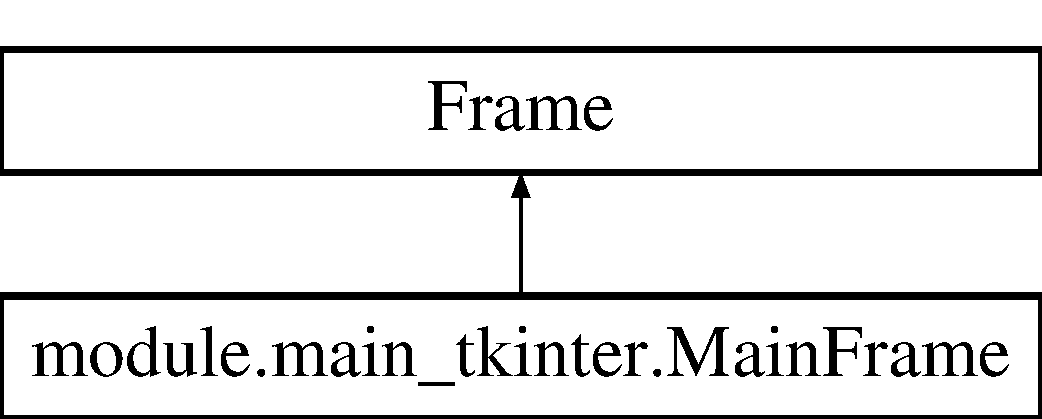
\includegraphics[height=2.000000cm]{classmodule_1_1main__tkinter_1_1_main_frame}
\end{center}
\end{figure}
\subsection*{Public Member Functions}
\begin{DoxyCompactItemize}
\item 
\mbox{\Hypertarget{classmodule_1_1main__tkinter_1_1_main_frame_aad46c64102fe51ec479d8b099e0f7db6}\label{classmodule_1_1main__tkinter_1_1_main_frame_aad46c64102fe51ec479d8b099e0f7db6}} 
def {\bfseries \+\_\+\+\_\+init\+\_\+\+\_\+} (self, parent, args, kwargs)
\end{DoxyCompactItemize}
\subsection*{Public Attributes}
\begin{DoxyCompactItemize}
\item 
\mbox{\Hypertarget{classmodule_1_1main__tkinter_1_1_main_frame_ae2685665dc8bf7b6af9bca1100272b2b}\label{classmodule_1_1main__tkinter_1_1_main_frame_ae2685665dc8bf7b6af9bca1100272b2b}} 
{\bfseries parent}
\item 
\mbox{\Hypertarget{classmodule_1_1main__tkinter_1_1_main_frame_a0e77ba421a2a0032e64ac56675b43b59}\label{classmodule_1_1main__tkinter_1_1_main_frame_a0e77ba421a2a0032e64ac56675b43b59}} 
{\bfseries label}
\item 
\mbox{\Hypertarget{classmodule_1_1main__tkinter_1_1_main_frame_af6b6e986fae014d58716a59704a0fd61}\label{classmodule_1_1main__tkinter_1_1_main_frame_af6b6e986fae014d58716a59704a0fd61}} 
{\bfseries close\+\_\+button}
\end{DoxyCompactItemize}


The documentation for this class was generated from the following file\+:\begin{DoxyCompactItemize}
\item 
/\+Users/apple/\+Documents/\+Git\+Hub/py-\/starter/module/main\+\_\+tkinter.\+py\end{DoxyCompactItemize}

\hypertarget{classmodule_1_1main__tkinter_1_1_script_frame}{}\section{module.\+main\+\_\+tkinter.\+Script\+Frame Class Reference}
\label{classmodule_1_1main__tkinter_1_1_script_frame}\index{module.\+main\+\_\+tkinter.\+Script\+Frame@{module.\+main\+\_\+tkinter.\+Script\+Frame}}
Inheritance diagram for module.\+main\+\_\+tkinter.\+Script\+Frame\+:\begin{figure}[H]
\begin{center}
\leavevmode
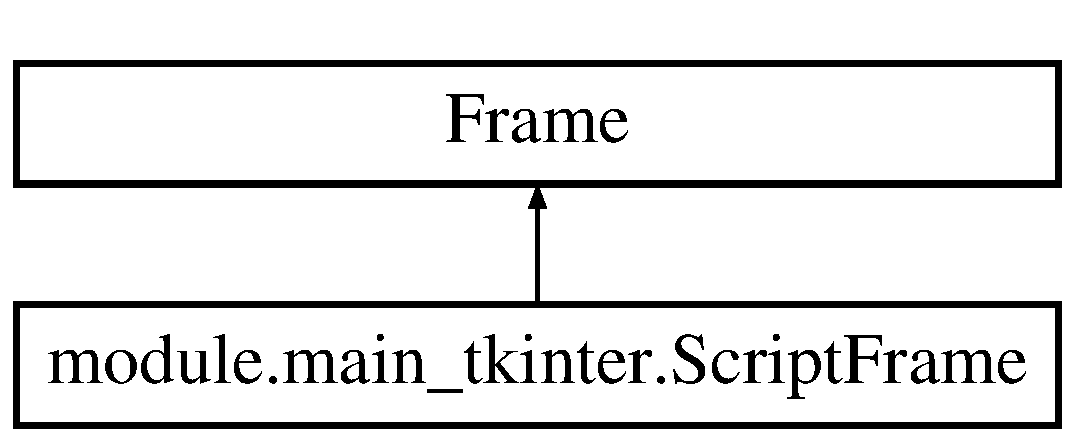
\includegraphics[height=2.000000cm]{classmodule_1_1main__tkinter_1_1_script_frame}
\end{center}
\end{figure}
\subsection*{Public Member Functions}
\begin{DoxyCompactItemize}
\item 
\mbox{\Hypertarget{classmodule_1_1main__tkinter_1_1_script_frame_a0237eba3d07ddab81cf156b9caa9f022}\label{classmodule_1_1main__tkinter_1_1_script_frame_a0237eba3d07ddab81cf156b9caa9f022}} 
def {\bfseries \+\_\+\+\_\+init\+\_\+\+\_\+} (self, parent, args, kwargs)
\end{DoxyCompactItemize}
\subsection*{Public Attributes}
\begin{DoxyCompactItemize}
\item 
\mbox{\Hypertarget{classmodule_1_1main__tkinter_1_1_script_frame_aea3087a23a015b744e6a2164518c08d7}\label{classmodule_1_1main__tkinter_1_1_script_frame_aea3087a23a015b744e6a2164518c08d7}} 
{\bfseries parent}
\item 
\mbox{\Hypertarget{classmodule_1_1main__tkinter_1_1_script_frame_a14ddfa23d3c3a020d4de18ce038f449b}\label{classmodule_1_1main__tkinter_1_1_script_frame_a14ddfa23d3c3a020d4de18ce038f449b}} 
{\bfseries script}
\end{DoxyCompactItemize}


The documentation for this class was generated from the following file\+:\begin{DoxyCompactItemize}
\item 
/\+Users/apple/\+Documents/\+Git\+Hub/py-\/starter/module/main\+\_\+tkinter.\+py\end{DoxyCompactItemize}

\hypertarget{classmodule_1_1main_1_1_test_app}{}\section{module.\+main.\+Test\+App Class Reference}
\label{classmodule_1_1main_1_1_test_app}\index{module.\+main.\+Test\+App@{module.\+main.\+Test\+App}}


This \mbox{\hyperlink{classmodule_1_1main_1_1_test_app}{Test\+App}} is sub-\/class of \char`\"{}kivy.\+app.\+App\char`\"{}.  


Inheritance diagram for module.\+main.\+Test\+App\+:\begin{figure}[H]
\begin{center}
\leavevmode
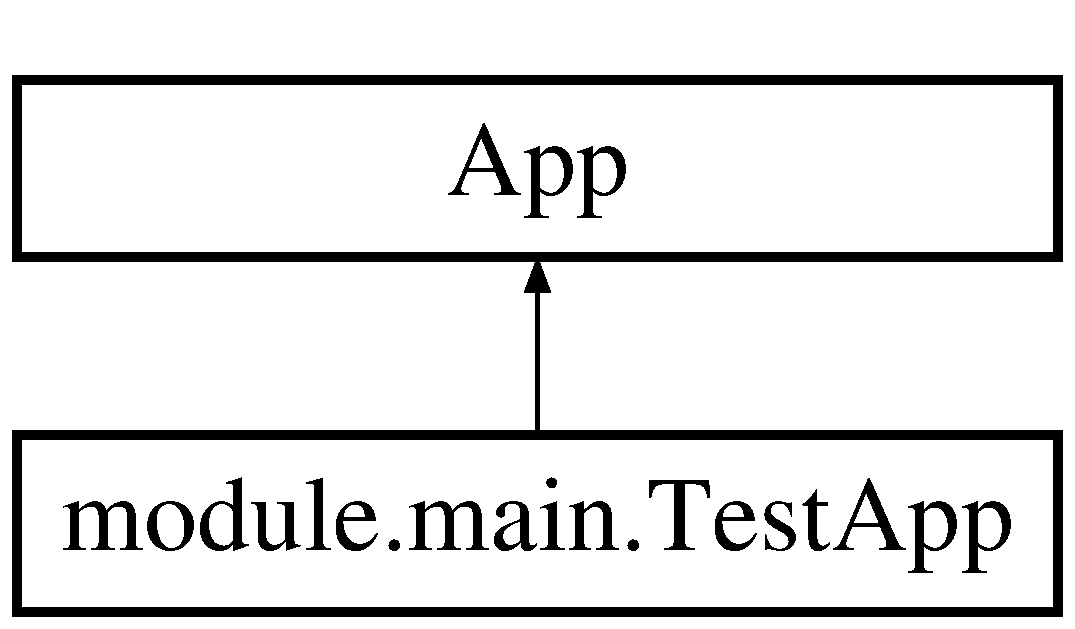
\includegraphics[height=2.000000cm]{classmodule_1_1main_1_1_test_app}
\end{center}
\end{figure}
\subsection*{Public Member Functions}
\begin{DoxyCompactItemize}
\item 
def \mbox{\hyperlink{classmodule_1_1main_1_1_test_app_a56f9c311e4db9ec9a313687f4c6d5faf}{build}} (self)
\begin{DoxyCompactList}\small\item\em This method is kivy.\+app.\+App.\+build(). \end{DoxyCompactList}\end{DoxyCompactItemize}


\subsection{Detailed Description}
This \mbox{\hyperlink{classmodule_1_1main_1_1_test_app}{Test\+App}} is sub-\/class of \char`\"{}kivy.\+app.\+App\char`\"{}. 

\subsection{Member Function Documentation}
\mbox{\Hypertarget{classmodule_1_1main_1_1_test_app_a56f9c311e4db9ec9a313687f4c6d5faf}\label{classmodule_1_1main_1_1_test_app_a56f9c311e4db9ec9a313687f4c6d5faf}} 
\index{module\+::main\+::\+Test\+App@{module\+::main\+::\+Test\+App}!build@{build}}
\index{build@{build}!module\+::main\+::\+Test\+App@{module\+::main\+::\+Test\+App}}
\subsubsection{\texorpdfstring{build()}{build()}}
{\footnotesize\ttfamily def module.\+main.\+Test\+App.\+build (\begin{DoxyParamCaption}\item[{}]{self }\end{DoxyParamCaption})}



This method is kivy.\+app.\+App.\+build(). 

~\newline
 Implementing its \mbox{\hyperlink{classmodule_1_1main_1_1_test_app_a56f9c311e4db9ec9a313687f4c6d5faf}{build()}} method, so it returns a Widget instance (the root of your widget tree) 

The documentation for this class was generated from the following file\+:\begin{DoxyCompactItemize}
\item 
/\+Users/apple/\+Documents/\+Git\+Hub/py-\/starter/module/main.\+py\end{DoxyCompactItemize}

%--- End generated contents ---

% Index
\backmatter
\newpage
\phantomsection
\clearemptydoublepage
\addcontentsline{toc}{chapter}{\indexname}
\printindex

\end{document}
